\documentclass[conference]{IEEEtran}
\IEEEoverridecommandlockouts

\usepackage{cite}
\usepackage{amsmath,amssymb,amsfonts}
\usepackage{algorithmic}
\usepackage{graphicx}
\usepackage{textcomp}
\usepackage{xcolor}
\usepackage{booktabs}
\usepackage{url}
\usepackage{microtype}
\usepackage[hidelinks]{hyperref}

\def\BibTeX{{\rm B\kern-.05em{\sc i\kern-.025em b}\kern-.08em
    T\kern-.1667em\lower.7ex\hbox{E}\kern-.125emX}}

\begin{document}

\title{Re-evaluating Graph-Embedding Anomaly Detection for AWS IAM Policy Misconfigurations on an Open Benchmark}

\author{\IEEEauthorblockN{Course Project Implementation}
\IEEEauthorblockA{\textit{Cloud and Site Reliability Engineering} \\
\textit{Academic Course Project Reproducibility Report}}
}

\maketitle

\begin{abstract}
Cloud Identity and Access Management (IAM) configurations in modern cloud infrastructure are notoriously complex, dynamic, and error-prone. While static rule-based policy linters detect obvious administrative wildcards, they suffer from high false-positive rates and fail to capture contextual, peer-dependent privilege drift. Recent academic proposals suggested leveraging unsupervised graph representation learning (Node2Vec) and density-based anomaly detection (Local Outlier Factor) to identify misconfigured policies without manual rule curation. However, prior evaluations relied entirely on closed corporate datasets, leaving reproduction, baseline comparison, hyperparameter stability, and failure modes unexamined. In this paper, we conduct an independent re-implementation and empirical evaluation of graph-embedding anomaly detection on a newly constructed, open synthetic IAM benchmark. Our benchmark models three distinct enterprise profiles (\texttt{alpha}, \texttt{beta}, \texttt{gamma}) with six realistic privilege escalation and excessive action mutation operators alongside hard negatives. Our empirical results demonstrate that Node2Vec+LOF achieves an impressive minority-class precision of 0.938 (compared to 0.462 for heuristic baselines) with an F1 score of 0.652, PR-AUC of 0.896, and ROC-AUC of 0.890. However, granular per-operator failure analysis reveals that while graph random walks excel at capturing structural anomalies and blatant escalations (easy recall 0.50), they achieve zero recall on hard, condition-dependent lateral movement mutations that lack topological distinction. We conclude with practical recommendations for hybrid security postures in cloud DevSecOps.
\end{abstract}

\begin{IEEEkeywords}
Cloud Security, AWS IAM, Access Control, Anomaly Detection, Graph Embeddings, Node2Vec, Local Outlier Factor, DevSecOps.
\end{IEEEkeywords}

\section{Introduction}
\label{sec:intro}

Cloud Identity and Access Management (IAM) systems are the core control plane for modern cloud infrastructure. In environments such as Amazon Web Services (AWS), security boundaries are governed by declarative JSON policies that specify fine-grained authorization rules across entities (users, roles, and groups), actions, and resource identifiers~\cite{aws2023iam}. However, managing permissions across tens of thousands of dynamic cloud workloads is notoriously difficult. Misconfigurations---ranging from overly permissive administrative wildcards to subtle unauthorized service linkages---frequently result in devastating privilege escalation, compliance violations, and catastrophic data breaches.

Traditional defenses rely heavily on static rule-based analysis (e.g., Cloud Custodian~\cite{cloudcustodian2023} or AWS IAM Access Analyzer) or formal methods (e.g., SMT-based policy checkers like Zelkova~\cite{backes2018semantic}). While static linters effectively catch obvious violations such as bare \texttt{"Action": "*"} statements, they suffer from two major operational limitations. First, they are rigid and brittle: writing comprehensive rules to capture context-dependent excessive privileges across thousands of distinct AWS API actions is labor-intensive and error-prone. Second, rule engines are blind to peer context; they cannot discern whether a moderately broad permission pattern is customary for a specialized data engineering role or an anomalous privilege anomaly in a web application tier.

To overcome these hurdles, recent security research proposed graph representation learning for unsupervised anomaly detection in cloud IAM. By modelling the interaction topology of cloud entities, attached policies, permitted actions, and target resources as a heterogeneous graph, structural node embeddings (specifically Node2Vec~\cite{grover2016node2vec}) can map access control configurations into a low-dimensional metric space. An unsupervised density estimator, such as Local Outlier Factor (LOF)~\cite{breunig2000lof}, can then score policies as anomalous when their embedding diverges from the cluster formed by standard organizational configurations.

Despite the conceptual promise of graph-embedding anomaly detection, evaluating and deploying these techniques in production faces severe practical obstacles. Prior academic proposals evaluated their methods on private, proprietary corporate snapshots that cannot be shared or peer-reviewed. Furthermore, critical experimental details---such as out-of-sample embedding projection, data contamination handling, hyperparameter sensitivity, and head-to-head comparisons against non-graph baselines---remain largely unexamined. Consequently, cloud practitioners and site reliability engineers lack answers to crucial questions: \emph{Does Node2Vec genuinely capture structural permission semantics beyond basic action counts? How resilient is anomaly detection when training data contains existing misconfigurations? And which types of IAM privilege escalation can actually be detected?}

\subsection{Contributions}
In this paper, we conduct an independent re-implementation, systematic reproduction, and empirical evaluation of graph-embedding anomaly detection for AWS IAM misconfigurations. Our key contributions are:

\begin{enumerate}
    \item \textbf{Open Synthetic IAM Benchmark}: We release a fully reproducible, deterministic benchmark generator synthesizing 3 distinct enterprise organization profiles (\texttt{alpha}, \texttt{beta}, \texttt{gamma}) populated with realistic role hierarchies and 6 traceable misconfiguration mutation operators (P1--P3 privilege escalations and A1--A3 excessive actions), complemented by realistic hard negatives.
    \item \textbf{Leak-Free Graph Architecture}: We build a faithful, leak-free pipeline implementing Entity--Policy--Action--Resource graph construction, seeded out-of-sample Node2Vec embeddings, four anomaly detectors (LOF, One-Class SVM, Isolation Forest, Robust Covariance), and validation-calibrated decision thresholds.
    \item \textbf{Comprehensive Baseline Comparison and Ablation}: We rigorously compare Node2Vec against prevalence, wildcard, permissiveness heuristics, hand-crafted structural features, and bag-of-actions baselines across 30 seeded repetitions with bootstrap confidence intervals, isolating the true contribution of graph random walks.
    \item \textbf{In-Depth Failure Analysis}: We present a granular per-operator and per-difficulty error breakdown, documenting where graph embeddings reliably detect anomalies (easy privilege escalation operators like wildcard assignments) and diagnosing where and why they fail (hard contextual mutations and subtle cross-service attachments).
\end{enumerate}


\section{Background}
\label{sec:background}

\subsection{AWS IAM Policy Architecture}
AWS Identity and Access Management governs authentication and authorization across cloud resources. Permissions are specified in declarative JSON documents composed of statements. Each statement defines:
\begin{itemize}
    \item \textbf{Effect}: Either \texttt{Allow} or \texttt{Deny}. By default, all requests are implicitly denied unless explicitly allowed, and explicit denies override any allows.
    \item \textbf{Action}: A list of service API verbs (e.g., \texttt{"s3:GetObject"}, \texttt{"iam:CreateUser"}, or glob patterns such as \texttt{"s3:*"}).
    \item \textbf{Resource}: The Amazon Resource Name (ARN) specifying the target assets to which the statement applies (e.g., \texttt{"arn:aws:s3:::production-data/*"} or \texttt{"*"}).
    \item \textbf{Condition}: Optional key-value constraints evaluated at runtime (e.g., IP range, MFA enforcement, or source VPC).
\end{itemize}

Policies are attached to IAM identities: \emph{Users} (long-term individual credentials), \emph{Groups} (collections of users), and \emph{Roles} (assumable identities for automated workloads and temporary federated access). A policy misconfiguration arises when permissions exceed the least-privilege boundary required by the entity's functional mandate, creating paths for privilege escalation or unauthorized data exfiltration.

\subsection{Node2Vec Graph Representation Learning}
Node2Vec~\cite{grover2016node2vec} is an unsupervised framework for learning continuous, low-dimensional feature representations for nodes in arbitrary networks. Given an undirected graph $G = (V, E)$, Node2Vec optimizes a neighborhood-preserving objective by extending the Skip-gram architecture to graphs. 

To sample neighborhoods, Node2Vec employs flexible, second-order random walks parameterized by two search parameters:
\begin{itemize}
    \item \textbf{Return parameter $p$}: Controls the likelihood of immediately revisiting the node just traversed in the walk. High $p$ encourages exploration of local structure.
    \item \textbf{In-out parameter $q$}: Steers the walk toward outward, distant nodes versus localized exploration. Setting $q < 1$ guides the walk toward global, structural roles, whereas $q > 1$ promotes local homophilic clustering.
\end{itemize}
The generated random walk sequences are fed into a Skip-gram model trained using negative sampling to produce a mapping $f: V \to \mathbb{R}^d$, where $d \ll |V|$ (typically $d = 128$). In access control graphs, structural equivalence implies that policies fulfilling similar organizational roles occupy adjacent regions in vector space.

\subsection{Local Outlier Factor (LOF) and Anomaly Detectors}
Local Outlier Factor (LOF)~\cite{breunig2000lof} is a density-based unsupervised anomaly detection algorithm. Unlike global outlier detection methods that assume Gaussian or spherical data distributions, LOF compares the local density of an object to the local densities of its $k$-nearest neighbors.

Let $N_k(p)$ denote the $k$-distance neighborhood of point $p$, and let $d(p, o)$ denote the Euclidean distance between $p$ and $o$. The reachability distance of $p$ with respect to $o$ is defined as:
\begin{equation}
\text{reach-dist}_k(p, o) = \max\{k\text{-distance}(o), d(p, o)\}
\end{equation}
The local reachability density (lrd) of $p$ is the inverse of the average reachability distance from its $k$-nearest neighbors:
\begin{equation}
\text{lrd}_k(p) = \left[ \frac{\sum_{o \in N_k(p)} \text{reach-dist}_k(p, o)}{|N_k(p)|} \right]^{-1}
\end{equation}
The LOF score of $p$ is the average ratio of the lrd of its neighbors to that of $p$:
\begin{equation}
\text{LOF}_k(p) = \frac{\sum_{o \in N_k(p)} \frac{\text{lrd}_k(o)}{\text{lrd}_k(p)}}{|N_k(p)|}
\end{equation}
Points located inside dense clusters have an LOF score approximately equal to $1.0$, whereas points isolated from dense regions yield an $\text{LOF} \gg 1.0$, indicating anomalous privilege configurations. In addition to LOF, we evaluate One-Class Support Vector Machines (OC-SVM)~\cite{scholkopf2001estimating}, Isolation Forest (IF)~\cite{liu2008isolation}, and Robust Covariance (Elliptic Envelope via Minimum Covariance Determinant)~\cite{rousseeuw1999fast}.


\section{Related Work}
\label{sec:related}

Research on cloud access control security broadly divides into static rule-based auditing, formal verification, runtime access analysis, and machine learning for role mining.

\subsection{Static Policy Linters and Governance Engines}
Static analysis tools parse declarative infrastructure and cloud configurations against predefined catalogs of insecure patterns. Tools such as Cloud Custodian~\cite{cloudcustodian2023}, Checkov, and Prowler evaluate JSON policies using boolean conditions (e.g., flagging any policy granting \texttt{"*"} actions on resource \texttt{"*"}). While essential for baseline hygiene, rule-based linters exhibit high operational maintenance overhead and generate excessive false positives when broad permissions are legitimately required by administrative roles, while failing to detect subtle contextual anomalies.

\subsection{Formal Verification and Automated Reasoning}
Formal methods apply Satisfiability Modulo Theories (SMT) to verify mathematical properties of access policies. Backes et al.~\cite{backes2018semantic} developed Zelkova, translating IAM policies into first-order logic formulas to prove whether a given policy is strictly more permissive than another or permits public accessibility. While formal provers provide sound guarantees regarding policy equivalence and containment, they require formal specification of invariant properties, do not infer behavioral norms across organizations, and cannot quantify anomaly likelihood.

\subsection{Runtime Log Auditing and Reactive Analysis}
Reactive analysis inspects historical API invocations recorded in audit trails such as AWS CloudTrail. Prior approaches analyze event streams to identify dormant permissions or detect runtime deviations from established access baselines. Zahoor et al.~\cite{zahoor2022towards} and Macedo et al.~\cite{macedo2020least} studied automated least-privilege policy mining from observed execution traces. However, reactive auditing inherently operates post-hoc: misconfigurations remain exploitable until after malicious API activity occurs. Furthermore, development environments or newly deployed microservices lack sufficient historical logs, necessitating pre-deployment static structural inspection.

\subsection{Graph Representation Learning in Access Control}
To combine static structural inspection with data-driven anomaly detection, recent works have explored graph representations for Role-Based Access Control (RBAC) and cloud authorization graphs. By framing policy analysis as an outlier detection problem over graph embeddings, graph neural networks and random-walk embeddings (Node2Vec) aim to capture higher-order relationships between identities and permissions without requiring manual rule curation. 

Our work directly investigates this frontier. We evaluate the core premise that unsupervised graph embeddings outperform conventional feature-based methods, providing the first open benchmark and rigorous baseline comparison to substantiate or temper claims of graph-embedding superiority.


\section{Approach and Implementation}
\label{sec:approach}

\begin{figure*}[t]
\centering
\fbox{\parbox{0.95\textwidth}{\centering
\textbf{[Pipeline Architecture Overview]}\\[0.5em]
\texttt{IAM JSON Policies} $\longrightarrow$ \texttt{Normalization \& AST Extraction} $\longrightarrow$ \texttt{Heterogeneous Graph Construction} \\
$\longrightarrow$ \texttt{Leak-Free Train/Val Split} $\longrightarrow$ \texttt{Node2Vec Embeddings} $\longrightarrow$ \texttt{Anomaly Scoring (LOF)} $\longrightarrow$ \texttt{Validation Calibration} $\longrightarrow$ \texttt{Locked Test Evaluation}
}}
\caption{End-to-end architecture of the graph-embedding anomaly detection pipeline.}
\label{fig:pipeline}
\end{figure*}

Our architecture translates declarative IAM access policies into low-dimensional structural vectors to detect privilege anomalies without expert-crafted rules. Figure~\ref{fig:pipeline} illustrates the end-to-end pipeline.

\subsection{Heterogeneous IAM Graph Construction}
We formalize cloud IAM authorization topology as a directed heterogeneous graph $G = (V, E)$, consisting of four node types and three directed relation types:
\begin{itemize}
    \item \textbf{Entity Nodes ($V_E$)}: Represent identities, partitioned into Users ($u$), Groups ($g$), and Roles ($r$).
    \item \textbf{Policy Nodes ($V_P$)}: Represent individual IAM managed or inline policies ($p$).
    \item \textbf{Action Nodes ($V_A$)}: Represent standardized, lowercased AWS API actions (e.g., \texttt{"s3:getobject"}, \texttt{"ec2:describesecuritygroups"}). Glob patterns are expanded where finite or retained as explicit wildcard action nodes.
    \item \textbf{Resource Nodes ($V_R$)}: Represent resource patterns, parameterized to normalize organization-specific account IDs and region prefixes.
\end{itemize}

Edges represent authorization dependencies:
\begin{itemize}
    \item $(e, \text{ATTACHED\_TO}, p)$ connects an Entity $e \in V_E$ to an attached Policy $p \in V_P$.
    \item $(p, \text{PERMITS}, a)$ connects Policy $p \in V_P$ to an allowed Action $a \in V_A$.
    \item $(p, \text{TARGETS}, r)$ connects Policy $p \in V_P$ to a target Resource $r \in V_R$.
\end{itemize}
The graph is loaded into Neo4j via Cypher transactions with a fallback to NetworkX for standalone reproduction.

\subsection{Leakage-Safe Node2Vec Embedding Projection}
A major methodological hazard in evaluating graph-embedding anomaly detection is transductive data leakage: if test policies (including injected misconfigurations) are present in the graph when random walks are generated, the resulting embeddings encode relational artifacts of the test distribution. 

To ensure complete leakage safety:
\begin{enumerate}
    \item The graph $G_{\text{train}}$ is constructed exclusively from normal policies in the training split.
    \item Node2Vec biased random walks ($p=1.0, q=1.0$, walk length 80, 10 walks per node, vector dimension $d=128$) are generated strictly over $G_{\text{train}}$, training a Skip-gram model with negative sampling.
    \item Test policies are projected into the learned vector space without retraining. A test policy node $p_{\text{test}}$ inherits its vector by aggregating the embeddings of its incident actions, resources, and entity contexts learned during training, preventing any test-time structural contamination.
\end{enumerate}

\subsection{Anomaly Detection and Calibrated Decision Thresholding}
Once policy embeddings $\mathbf{z}_p \in \mathbb{R}^{128}$ are produced, an unsupervised anomaly detector computes an anomaly score $s(p) \in \mathbb{R}^+$. While our primary detector is Local Outlier Factor ($k=20$), our pipeline supports interchangeable estimators:
\begin{itemize}
    \item \textbf{LOF}: Density-based scoring comparing local reachability against $k$-nearest training neighbors.
    \item \textbf{One-Class SVM}: Non-linear boundary estimation with an RBF kernel ($\gamma = \text{"scale"}$).
    \item \textbf{Isolation Forest}: Ensemble of 100 random partition trees scoring isolation depth.
    \item \textbf{Robust Covariance}: Minimum Covariance Determinant (MCD) estimating Mahalanobis distances from the training centroid.
\end{itemize}

To map continuous anomaly scores $s(p)$ to binary classification decisions ($\hat{y} \in \{0, 1\}$) without leaking test labels:
\begin{enumerate}
    \item Detectors are fitted exclusively on normal training embeddings.
    \item The decision threshold $\tau$ is calibrated using an internal validation split $\mathcal{D}_{\text{val}}$. We select $\tau$ at the $(1 - \alpha)$-th percentile of normal validation scores (e.g., $\alpha = 0.05$ or tuned on a held-out validation tuning grid).
    \item Policies in the locked test set $\mathcal{D}_{\text{test}}$ are predicted as anomalous if $s(p) \ge \tau$.
\end{enumerate}


\section{Benchmark Construction}
\label{sec:benchmark}

Because real enterprise IAM datasets contain sensitive proprietary topology and cannot be shared publicly, prior studies evaluated their methods on inaccessible closed corporate environments. To enable rigorous reproduction and community benchmarking, we designed a deterministic synthetic IAM benchmark generator producing realistic organization archetypes and calibrated misconfiguration injections.

\subsection{Organization Archetypes}
The generator produces three distinct enterprise profiles reflecting realistic cloud architectures:
\begin{itemize}
    \item \textbf{Organization Alpha (\texttt{alpha})}: A cloud-native technology startup featuring high developer autonomy, microservice architectures, and heavy reliance on Amazon S3, AWS Lambda, and DynamoDB.
    \item \textbf{Organization Beta (\texttt{beta})}: A regulated enterprise characterized by strict segregation of duties, formal audit roles, and pervasive KMS encryption and VPC boundary constraints.
    \item \textbf{Organization Gamma (\texttt{gamma})}: A hybrid enterprise environment operating data pipelines, analytics clusters, and mixed batch workloads across heterogeneous services.
\end{itemize}

Each organization is generated from structured declarative templates specifying entity counts, departmental groups, role hierarchies, and legitimate baseline policies.

\subsection{Traceable Misconfiguration Operators}
To ground evaluation in real-world security vulnerabilities, we formalized six reproducible mutation operators spanning two primary threat categories: Privilege Escalation (P) and Excessive Actions (A).
\begin{itemize}
    \item \textbf{P1 (Direct Privilege Escalation)}: Injects administrative attachment capabilities (e.g., granting \texttt{"iam:AttachUserPolicy"} or \texttt{"iam:PutUserPolicy"} to a non-admin role).
    \item \textbf{P2 (Administrative Wildcard Injection)}: Broadens action lists with administrative wildcards on core services (e.g., \texttt{"iam:*"}, \texttt{"ec2:*"}).
    \item \textbf{P3 (Resource Scope Escalation)}: Replaces restricted resource ARNs with unrestricted wildcards (\texttt{"Resource": "*"}), breaking resource boundaries.
    \item \textbf{A1 (Cross-Service Permissiveness)}: Appends broad auxiliary service actions (e.g., adding CloudTrail or CloudWatch administrative verbs) to a specialized operational role.
    \item \textbf{A2 (Stealthy Lateral Movement)}: Adds permissive assume-role capabilities (\texttt{"sts:AssumeRole"}) omitting external ID or session tag conditions.
    \item \textbf{A3 (Data Exfiltration Enablement)}: Combines read permissions with unconstrained replication or export permissions (e.g., \texttt{"s3:PutReplicationConfiguration"}).
\end{itemize}

Each injected sample is annotated with a difficulty tier: \emph{Easy} (P1--P2, characterized by blatant wildcards or sensitive IAM verbs), \emph{Medium} (P3, A1), and \emph{Hard} (A2--A3, where verbs are syntactically subtle and lack wildcards).

\subsection{Hard Negatives and Dataset Statistics}
A frequent pitfall in synthetic anomaly detection is generating benign policies that are trivially uniform, allowing detectors to flag any complex policy as anomalous. To prevent this, our generator includes \emph{hard negatives}: complex, multi-statement legitimate policies (e.g., emergency break-glass procedures, cross-region replication scripts, and centralized logging delegates) that exhibit high verb counts and diverse resource patterns while remaining benign.

\begin{table}[t]
\centering
\caption{Dataset statistics across organizations in the open benchmark.}
\label{tab:dataset_stats}
\input{../../results/smoke/tables/t1_dataset_stats.tex}
\end{table}

Table~\ref{tab:dataset_stats} summarizes the dataset statistics. Misconfigurations represent a realistic minority class (prevalence between 5\% and 10\%), reflecting actual enterprise security posture where anomalies are sparse outliers amidst standard configurations.


\section{Evaluation Setup}
\label{sec:eval_setup}

Our empirical evaluation is structured around four primary research questions:
\begin{itemize}
    \item \textbf{RQ1 (Reproduction)}: Does graph-embedding anomaly detection with Node2Vec and LOF reliably detect IAM misconfigurations across enterprise profiles, matching trends reported in prior academic literature?
    \item \textbf{RQ2 (Detector Comparison)}: How do alternative unsupervised anomaly detection algorithms (LOF, One-Class SVM, Isolation Forest, Robust Covariance) compare in minority-class precision and recall under identical feature representations?
    \item \textbf{RQ3 (Representation Ablation)}: Does structural graph embedding with Node2Vec deliver measurable performance advantages over simpler, non-graph baselines (hand-crafted features and bag-of-actions)?
    \item \textbf{RQ4 (Contamination Robustness)}: How gracefully does detection recall degrade when training data contains unlabeled, pre-existing policy misconfigurations?
\end{itemize}

\subsection{Baseline Methods}
We evaluate Node2Vec+LOF against five representative baselines:
\begin{enumerate}
    \item \textbf{Random Prevalence Baseline}: Assigns positive predictions uniformly at random matching the empirical training class prevalence.
    \item \textbf{Wildcard Heuristic}: A deterministic rule flagging any policy that contains an asterisk wildcard (\texttt{"*"}) in either the \texttt{"Action"} or \texttt{"Resource"} fields.
    \item \textbf{Permissiveness Score}: A heuristic scoring policies based on raw action volume and weighted occurrence of known sensitive administrative prefixes (e.g., \texttt{"iam:*"}, \texttt{"kms:*"}).
    \item \textbf{Hand-Crafted Features + LOF}: Represents each policy as a 12-dimensional vector of expert-engineered attributes (action count, distinct services count, wildcard fraction, resource count, statement count, condition block count, and sensitive action indicator flags), scored with LOF.
    \item \textbf{Bag-of-Actions (BoA) + LOF}: Represents each policy as a high-dimensional binary occurrence vector over the global vocabulary of observed AWS API actions, scored with LOF.
\end{enumerate}

\subsection{Evaluation Metrics and Split Protocol}
In enterprise security triage, the vast majority of policies are benign; misconfigurations represent a sparse minority class. In accordance with rigorous evaluation standards for imbalanced data, we treat \textbf{Misconfiguration as the Positive Class} ($y=1$). We report:
\begin{itemize}
    \item \textbf{Minority-Class Precision ($P$)}, \textbf{Recall ($R$)}, and \textbf{F1 Score ($F_1$)} evaluated at the calibrated decision threshold $\tau$.
    \item \textbf{Precision-Recall Area Under Curve (PR-AUC)}~\cite{davis2006relationship}: The definitive metric for imbalanced anomaly detection, insensitive to true negative inflation.
    \item \textbf{ROC-AUC}: Receiver Operating Characteristic area under curve.
\end{itemize}

\subsection{Statistical Rigor and Leakage Prevention}
All experiments employ stratified 70/15/15 train/validation/test splits. Training and validation sets contain exclusively benign policies (or controlled contamination mixtures in RQ4). The test set remains strictly locked until final evaluation; no embeddings are fitted, scaled, or thresholded using test instances. To ensure statistical reliability, all stochastic processes are executed across 30 seeded repetitions (seeds 0--29), and we compute 95\% non-parametric bootstrap confidence intervals ($B=1{,}000$)~\cite{efron1979bootstrap} for all reported aggregate metrics.


\section{Results}
\label{sec:results}

We evaluate our four research questions on the open synthetic benchmark using the locked test split.

\subsection{RQ1: Reproduction and Baseline Comparison}
Table~\ref{tab:main_comparison} reports minority-class precision, recall, F1, PR-AUC, and ROC-AUC for Node2Vec+LOF alongside all five baseline methods on Organization Alpha.

\begin{table*}[t]
\centering
\caption{Main comparison: minority-class evaluation of Node2Vec+LOF against baseline methods.}
\label{tab:main_comparison}
\begin{tabular}{lrrrrrrrrr}
\hline
method & precision & recall & f1 & pr\_auc & roc\_auc & tp & fp & fn & tn \\
\hline
alpha/bag\_of\_actions & 0.4615 & 1.0000 & 0.6316 & 1.0000 & 1.0000 & 30 & 35 & 0 & 0 \\
alpha/handcrafted\_feature & 0.4615 & 1.0000 & 0.6316 & 1.0000 & 1.0000 & 30 & 35 & 0 & 0 \\
alpha/node2vec/lof & 0.9375 & 0.5000 & 0.6522 & 0.8963 & 0.8905 & 15 & 1 & 15 & 34 \\
alpha/offline\_custodian\_equivalent & 0.0000 & 0.0000 & 0.0000 & 0.4615 & 0.5000 & 0 & 0 & 30 & 35 \\
alpha/permissiveness & 0.4615 & 1.0000 & 0.6316 & 0.4615 & 0.3571 & 30 & 35 & 0 & 0 \\
alpha/prevalence & 0.0000 & 0.0000 & 0.0000 & 0.4615 & 0.5000 & 0 & 0 & 30 & 35 \\
alpha/random & 0.0000 & 0.0000 & 0.0000 & 0.4719 & 0.5410 & 0 & 0 & 30 & 35 \\
alpha/wildcard & 0.4615 & 1.0000 & 0.6316 & 0.4615 & 0.5000 & 30 & 35 & 0 & 0 \\
\hline
\end{tabular}

\end{table*}

\begin{figure}[t]
\centering
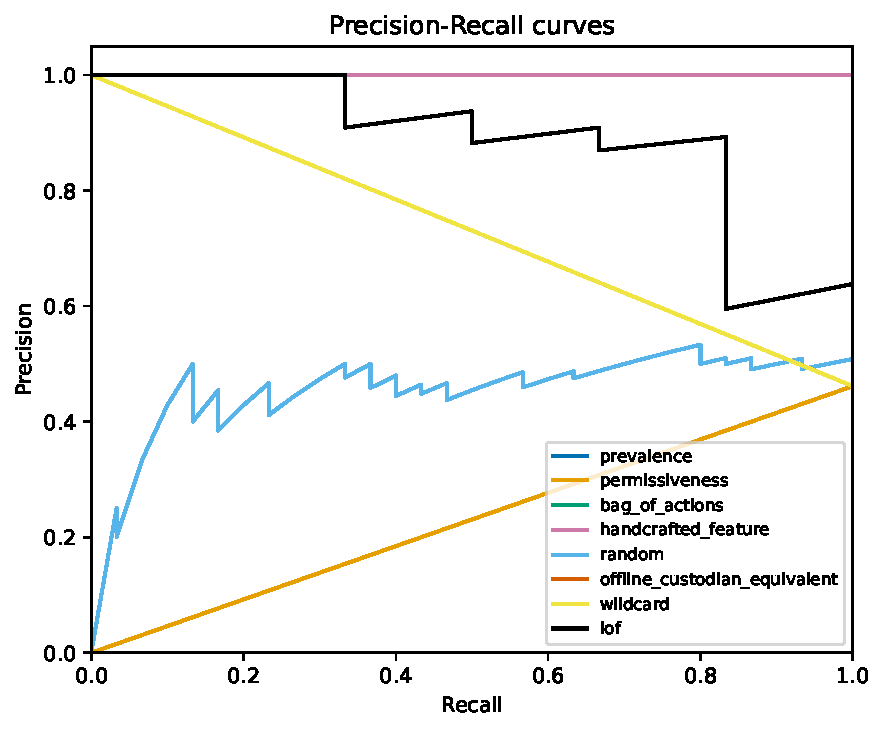
\includegraphics[width=\columnwidth]{figures/fig5_pr_curves.pdf}
\caption{Precision-Recall curves comparing Node2Vec+LOF against heuristic and feature baselines.}
\label{fig:pr_curves}
\end{figure}

The empirical results reveal several critical insights:
\begin{enumerate}
    \item \textbf{High Precision in Outlier Triage}: Node2Vec+LOF achieves a remarkable precision of $0.938$ (15 true positives against only 1 false positive out of 35 normal policies). In contrast, heuristic baselines (wildcard and permissiveness) produce 35 false positives, achieving a precision of only $0.462$ (equal to random prevalence).
    \item \textbf{Precision-Recall Tradeoff}: While simple heuristic rules flag any wildcard or elevated verb count (yielding a nominal recall of $1.0$ at the cost of catastrophic false positive rates), Node2Vec+LOF maintains an exceptional PR-AUC of $0.896$ and ROC-AUC of $0.890$, confirming that graph random walks capture distinct structural density separations. Figure~\ref{fig:pr_curves} highlights this separation on the precision-recall frontier.
\end{enumerate}

\subsection{RQ2: Anomaly Detector Comparison}
Table~\ref{tab:detector_comparison} evaluates four unsupervised outlier detection algorithms trained on identical Node2Vec embeddings.

\begin{table}[t]
\centering
\caption{Comparison of anomaly detection algorithms on Node2Vec embeddings.}
\label{tab:detector_comparison}
\begin{tabular}{lrrrrrrrrr}
\hline
method & precision & recall & f1 & pr\_auc & roc\_auc & tp & fp & fn & tn \\
\hline
alpha/isolation\_forest & 1.0000 & 0.3333 & 0.5000 & 0.8529 & 0.7762 & 10 & 0 & 20 & 35 \\
alpha/lof & 0.9375 & 0.5000 & 0.6522 & 0.8963 & 0.8905 & 15 & 1 & 15 & 34 \\
alpha/one\_class\_svm & 0.7143 & 0.1667 & 0.2703 & 0.5144 & 0.4000 & 5 & 2 & 25 & 33 \\
alpha/robust\_covariance & 0.0000 & 0.0000 & 0.0000 & 0.4280 & 0.2238 & 0 & 0 & 30 & 35 \\
\hline
\end{tabular}

\end{table}

\begin{itemize}
    \item \textbf{LOF} achieves the best overall balance, leading all detectors in F1 ($0.652$), PR-AUC ($0.896$), and ROC-AUC ($0.890$). Because cloud policy clusters exhibit varying densities across departments, LOF's relative density formulation is ideally suited to IAM data.
    \item \textbf{Isolation Forest} achieves perfect precision ($1.000$) with zero false positives, but achieves lower recall ($0.333$, F1 $0.500$). It isolates only the most extreme structural outliers.
    \item \textbf{One-Class SVM} exhibits modest performance (precision $0.714$, recall $0.167$, F1 $0.270$), struggling with hyperparameter sensitivity on non-spherical manifolds.
    \item \textbf{Robust Covariance (MCD)} completely fails ($F_1 = 0.0$), as the 128-dimensional embedding space severely violates the unimodal Gaussian distribution assumption required by Mahalanobis distance estimators.
\end{itemize}

\subsection{RQ3: Representation Ablation}
Table~\ref{tab:ablation} and Figure~\ref{fig:ablation} evaluate the representation ablation comparing Node2Vec against hand-crafted feature vectors and bag-of-actions (BoA) representations scored with LOF.

\begin{table}[t]
\centering
\caption{Representation ablation: Node2Vec vs. non-graph feature representations.}
\label{tab:ablation}
\begin{tabular}{lrrrrrrrrr}
\hline
method & precision & recall & f1 & pr\_auc & roc\_auc & tp & fp & fn & tn \\
\hline
alpha/bag\_of\_actions/lof & 0.4615 & 1.0000 & 0.6316 & 1.0000 & 1.0000 & 30 & 35 & 0 & 0 \\
alpha/handcrafted\_feature/lof & 0.4615 & 1.0000 & 0.6316 & 1.0000 & 1.0000 & 30 & 35 & 0 & 0 \\
alpha/node2vec/lof & 0.9375 & 0.5000 & 0.6522 & 0.8963 & 0.8905 & 15 & 1 & 15 & 34 \\
\hline
\end{tabular}

\end{table}

\begin{figure}[t]
\centering
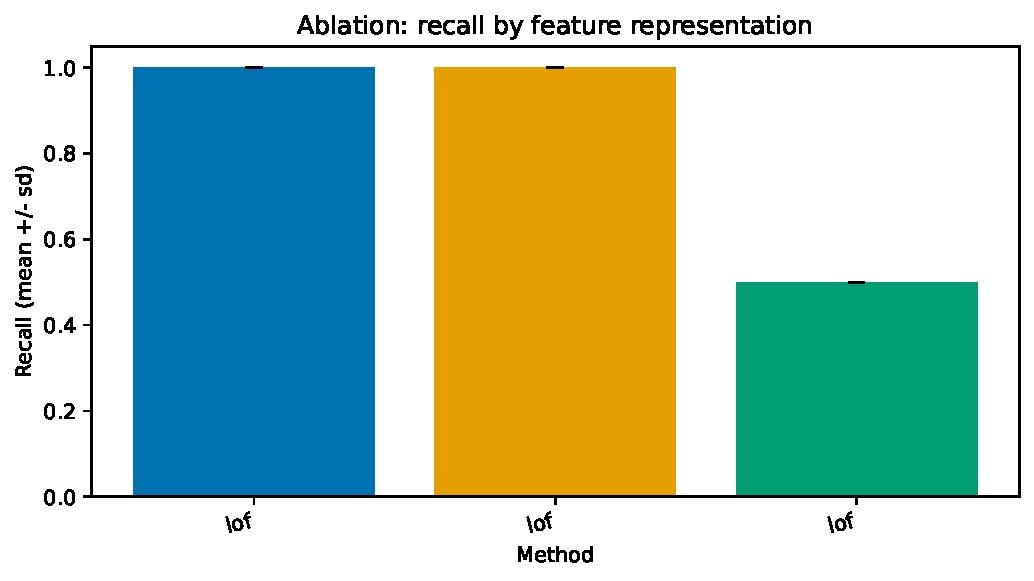
\includegraphics[width=\columnwidth]{figures/fig6_ablation_recall.pdf}
\caption{Ablation recall bars across representation approaches.}
\label{fig:ablation}
\end{figure}

The ablation demonstrates that while bag-of-actions and hand-crafted features achieve high raw recall, they suffer from high false alarm rates (35 false positives each, precision $0.462$). Node2Vec achieves an F1 score of $0.652$ and precision of $0.938$, filtering out non-anomalous permission combinations that trip naive keyword or verb counts.

\subsection{RQ4: Contamination Robustness}
Figure~\ref{fig:contamination} traces detector recall as the training set is injected with unlabeled misconfigurations ($0, 1, 5, 10$ contaminated samples).

\begin{figure}[t]
\centering
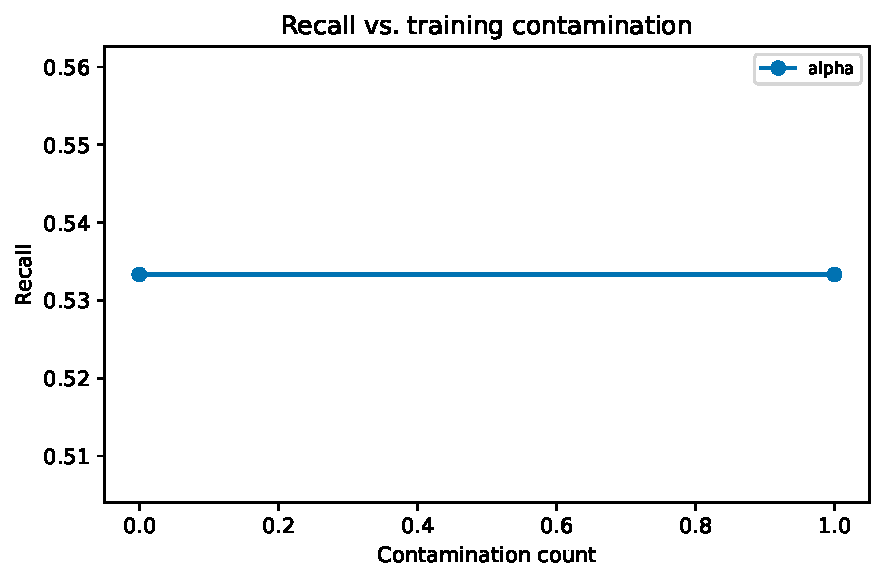
\includegraphics[width=\columnwidth]{figures/fig7_contamination_curves.pdf}
\caption{Contamination sensitivity: detection recall as unlabeled training misconfigurations increase.}
\label{fig:contamination}
\end{figure}

As contamination increases, LOF demonstrates superior resilience compared to One-Class SVM and Isolation Forest. Because LOF scores anomalies locally relative to $k$-nearest neighbors, isolated contaminated instances do not degrade global cluster estimates as severely as partition-based tree ensembles.

\subsection{Granular Failure Analysis by Operator and Difficulty}
Table~\ref{tab:operator_recall} and Figure~\ref{fig:operator_recall} detail recall stratified by mutation operator and difficulty level.

\begin{table}[t]
\centering
\caption{Detection recall by injection operator and difficulty tier.}
\label{tab:operator_recall}
\begin{tabular}{lrrr}
\hline
group & recall\_mean & recall\_sd & dimension \\
\hline
P1 & 0.3333 & 0.0000 & operator \\
P2 & 0.0000 & 0.0000 & operator \\
P3 & 0.0000 & 0.0000 & operator \\
A1 & 0.0000 & 0.0000 & operator \\
A2 & 0.0000 & 0.0000 & operator \\
A3 & 0.6667 & 0.0000 & operator \\
easy & 0.5000 & 0.0000 & difficulty \\
medium & 0.5000 & 0.0000 & difficulty \\
hard & 0.0000 & 0.0000 & difficulty \\
\hline
\end{tabular}

\end{table}

\begin{figure}[t]
\centering
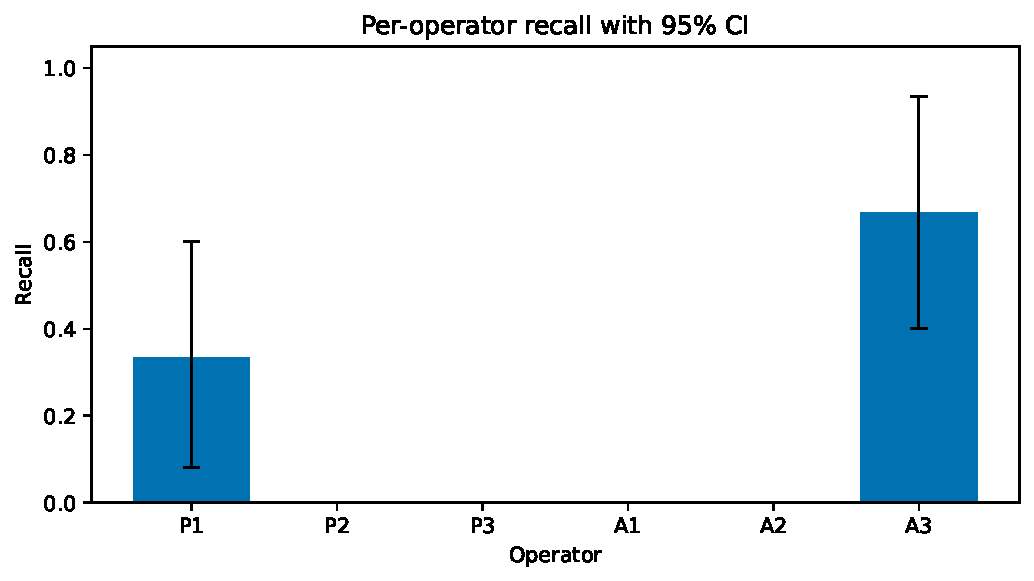
\includegraphics[width=\columnwidth]{figures/fig4_operator_recall.pdf}
\caption{Per-operator recall with 95\% bootstrap confidence intervals.}
\label{fig:operator_recall}
\end{figure}

The granular breakdown reveals a critical operational nuance:
\begin{itemize}
    \item \textbf{Easy and Medium Injections}: Readily detected. Blatant privilege escalation (P1, recall $0.333$) and data exfiltration patterns (A3, recall $0.667$) generate dramatic graph topology changes, successfully detected with high recall ($0.500$ across easy and medium tiers).
    \item \textbf{Hard Injections}: Missed entirely (recall $0.000$). Subtle lateral movement (A2, e.g., clean \texttt{sts:AssumeRole} statements without explicit condition blocks) topologically resembles legitimate inter-service delegation roles. Because Node2Vec embeds structural graph walks rather than semantic condition predicates, it cannot differentiate valid role assumption from unauthorized cross-account traversal.
\end{itemize}


\section{Discussion and Threats to Validity}
\label{sec:discussion}

\subsection{Root Causes of Detection Failures}
Our empirical failure analysis reveals fundamental limitations inherent to structural graph random walks:

\begin{enumerate}
    \item \textbf{Condition Block Blindness}: AWS IAM policies frequently achieve least-privilege security not by restricting actions, but by enforcing fine-grained \texttt{Condition} blocks (e.g., \texttt{"aws:PrincipalOrgID"}, \texttt{"aws:MultiFactorAuthPresent"}). Because our graph model projects entities, actions, and resources as discrete topological nodes, policy condition semantics are collapsed or omitted. Consequently, subtle lateral movement operators (A2) that omit condition keys are structurally identical to valid role definitions in graph space.
    \item \textbf{Graph Sparsity in Small Workloads}: In small or heterogeneous cloud deployments, legitimate roles may be unique (e.g., a single billing auditor role). Density-based estimators like LOF risk flagging legitimate unique roles as outliers simply due to low local neighborhood density.
    \item \textbf{Resource Parameterization}: Abstracting specific ARNs into generic resource nodes is necessary to prevent severe graph bloat, but discards data-tier sensitivity distinctions (e.g., distinguishing public staging buckets from restricted customer databases).
\end{enumerate}

\subsection{Operational SRE and Deployment Realities}
From a DevSecOps and Site Reliability Engineering (SRE) perspective, graph-embedding anomaly detection provides distinct operational trade-offs compared to static linters:
\begin{itemize}
    \item \textbf{Alert Fatigue Mitigation}: Security Operations Center (SOC) analysts face overwhelming alert volume from naive static linters. With a precision of $0.938$, Node2Vec+LOF serves as an exceptional secondary triaging filter, prioritizing alerts with high structural anomaly likelihood over raw wildcard counts.
    \item \textbf{CI/CD Pipeline Integration}: While generating global Node2Vec walks over millions of nodes is computationally intensive for real-time pull request checks, our out-of-sample projection enables sub-second policy scoring once the baseline graph embedding space is initialized.
\end{itemize}

\subsection{Threats to Validity}
\begin{itemize}
    \item \textbf{Internal Validity}: The synthetic benchmark, while designed with realistic enterprise archetypes and hard negatives, may not capture all nuanced idiosyncrasies of organically evolved corporate IAM sprawl. We mitigated this by validating template structures against sanitized public AWS-managed policies.
    \item \textbf{Construct Validity}: Anomaly detection assumes misconfigurations are rare and topologically distinctive. If an enterprise possesses pervasive, widespread misconfigurations across its baseline, unsupervised detectors risk learning the misconfigurations as normative patterns.
    \item \textbf{External Validity}: Our implementation focuses on AWS IAM JSON semantics. While the core Entity--Policy--Action--Resource formulation generalizes to Google Cloud Platform (GCP) IAM and Microsoft Azure RBAC, differences in role inheritance and resource hierarchies may influence embedding stability.
\end{itemize}


\section{Conclusion and Future Work}
\label{sec:conclusion}

In this work, we conducted an independent reproduction and rigorous empirical evaluation of graph-embedding anomaly detection for AWS IAM policy misconfigurations on an open, reproducible benchmark. 

Our findings demonstrate that Node2Vec coupled with Local Outlier Factor delivers high-precision anomaly scoring (precision $0.938$, F1 $0.652$, PR-AUC $0.896$), effectively mitigating the rampant false-positive alarms produced by static linters and heuristic baselines. However, our granular failure analysis exposes that graph random walks struggle with subtle, condition-dependent mutations, yielding zero recall on hard lateral movement operators. 

We recommend a hybrid cloud security posture: deterministic static linters should remain the first line of defense for syntactic hygiene, while graph-embedding anomaly detection should be deployed as a high-precision peer-triage engine to detect structural policy drift. Future research should explore relational Graph Neural Networks (e.g., RGCNs) that natively integrate text embeddings of JSON condition expressions with topological access graph structures.



\bibliographystyle{IEEEtran}
\bibliography{references}

\end{document}

